\chapter{Data and Lab Setup}
\thispagestyle{plain}
\label {Data Lab Setup}
\section{Hardware}
We used $Samsung\ Galaxy\ Nexus$ mobile phone for conducting all experiments. The hardware and software specs are mentioned in Table ~\ref{table:samsung_galexy_nexsus}.
\begin{table}[htbp]
\caption{Test Device Hardware Specs}
\bigskip
\label{table:samsung_galexy_nexsus}
\centering
\begin{center}
\begin{tabular}{|c|c|}
\hline
Features & Samsung\ Galaxy\ Nexus \\ \hline
Operating System & Andriod 4.2 (Rooted) \\ \hline
Main Memory & 1024 MB \\ \hline
Processor & Dual core, 1200 MHz, ARM Cortex-A9 \\ \hline
Battery Capacity  & 1750 mAh \\ \hline
Wifi & 802.11 a, b, g, n \\ \hline
Sensors & GPS, Proximity, Accelerometer, Gyroscope, Compass, Barometer \\ \hline
\end{tabular}
\end{center}
\end{table}
\section{Data Set and Feature Selection}
For our analysis, we use Malware Genome Data Set~\cite{54}. The data set consists of 38 malware families and 925 malicious applications. Table~\ref{genome_data_table} on page~\pageref{genome_data_table} provides information regarding malware family and associated number samples. We selected 25 benign applications from various application areas such as Travel, Food, Entertainment, Finance and Games. These applications are listed in Table~\ref{benign_apps}. 

As discussed earlier in section~\ref{System Input} on page~\pageref{System Input} we used our system to generate the normalized dataset for 600 malicious and 25 benign applications. For our analysis, feature selection is done using sparseLDA normalization algorithm. Table ~\ref{table:selected_features} shows all the features that we selected for model building. After feature selection, data set is normalized using Zscore normalization method. This normalized data set is the base data set for various classifiers that we evaluated. The overall data pipeline is shown in the figure~\ref{method_andriod_data_pipeline}.

\begin{table}
\caption{Slected Feature Set}
\bigskip
\label{table:selected_features} 
\centering
\begin{center}
\begin{tabular}{|c|c|c|c|}
\hline
\_llseek   &  access   &  bind   & cacheflush   \\ \hline
chmod   &  clock\_gettime   & clock\_nanosleep   &  clone  \\ \hline
close   & connect   &  dup   &  epoll\_ctl   \\ \hline  
epoll\_wait   &  exit\_group   &  fchown32 & fcntl64     \\ \hline  
fdatasync   &  flock   & fork   &  fstat64   \\ \hline  
fsync  & futex   &  getdents64   &  getpid   \\ \hline  
getpriority   &  getsockname   &  getsockopt  & gettid   \\ \hline  
gettimeofday   &  getuid32   & ioctl   &  kill  \\ \hline  
listen   & lseek   &  lstat64   &  madvise   \\ \hline  
mkdir   &  mmap2   &  mprotect  &	munmap   \\ \hline  
nanosleep   &  open   & pipe   &  poll \\ \hline  
prctl   & pread   &  pwrite   &  read   \\ \hline  
recvfrom   &  rename   &  restart\_syscall   & rmdir  \\ \hline  
rt\_sigreturn   &  sched\_yield  & sendto   &  setpriority   \\ \hline  
setsockopt   & shutdown   &  sigprocmask   &  socket   \\ \hline  
socketpair   &  stat64   &  statfs64   & tgkill  \\ \hline  
umask   &  uname	& unlink   &	write \\ \hline
writev  & & & \\ \hline
\end{tabular}
\end{center}
\end{table}

\section{Experiments}

\begin{figure}[htp]
\centering
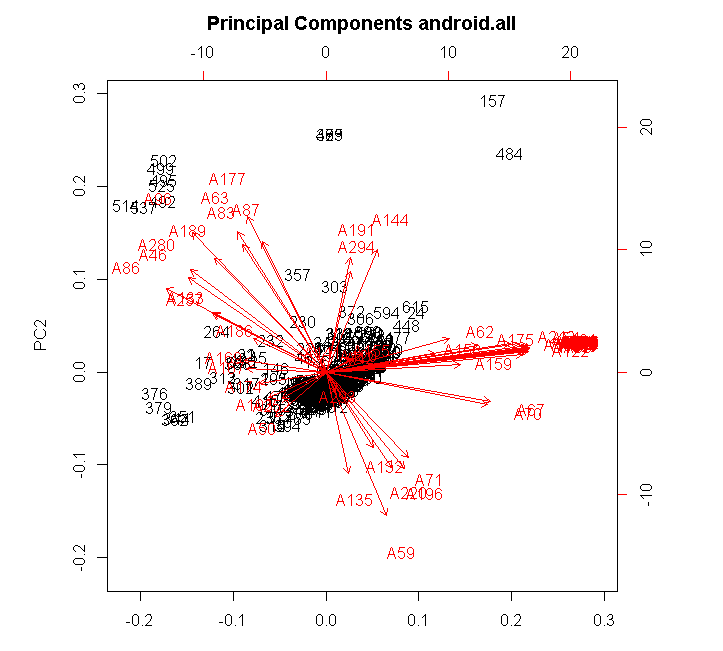
\includegraphics[width=\textwidth, height=0.6\textheight, keepaspectratio] {pca_analysis}
\caption{Principle components of data set using SVD method}
\bigskip
\label{fig:pca_analysis}
\end{figure}

For all experiments, we partitioned data set into training set (70\%) and testing set (30\%).  All models were evaluated for training error, test error and overall error rate. Figure ~\ref{fig:pca_analysis} shows the principle components of data set using svd method. Here we can observe that data set is densely clustered. Due to this classification problem becomes challenging.
\begin{table}[htp]
\caption{Malware Genome Project Dataset}
\label{genome_data_table} 
\bigskip
\centering
\begin{center}
\begin{tabular}{|l|r|l|r|l|r|}
\hline
TotalFamilies		&38&&&& 	\\ \hline
TotalSamples		&925&&&& 	\\ \hline
\hline
Malware Family & \# & Malware Family	& \#  & Malware Family & \# \\ \hline
ADRD				& 22  	&    Asroot				& 8  	&    BaseBridge			& 122  	\\ \hline
BeanBot				& 8  	&    Bgserv				& 9  	&    CruseWin			& 2  	\\ \hline
DogWars				& 1  	&    DroidCoupon		& 1  	&    DroidDeluxe		& 1  	\\ \hline
DroidDreamLight		& 46  	&    DroidKungFu1		& 34  	&    DroidKungFu2		& 30  	\\ \hline
DroidKungFu3		& 309  	&    DroidKungFu4		& 96  	&    DroidKungFuUpdate	& 1  	\\ \hline
Endofday			& 1  	&    FakeNetflix		& 1  	&    FakePlayer			& 6  	\\ \hline
GPSSMSSpy			& 6  	&    GamblerSMS			& 1  	&    Geinimi			& 18  	\\ \hline
GingerMaster		& 4  	&    GoldDream			& 47  	&    HippoSMS			& 4  	\\ \hline
Jifake				& 1  	&    LoveTrap			& 1  	&    Pjapps				& 58  	\\ \hline
Plankton			& 11  	&    RogueLemon			& 2  	&    RogueSPPush		& 9  	\\ \hline
SndApps				& 10  	&    Spitmo				& 1  	&    Tapsnake			& 2  	\\ \hline
Walkinwat			& 1  	&    Zitmo				& 1  	&    Zsone				& 12  	\\ \hline
zHash				& 11  	&   					&		&						&		\\ \hline
\end{tabular}
\end{center}
\end{table}

\begin{table}[htp]
\caption{Benign Android Applications}
\label{benign_apps}
\bigskip
\centering
\begin{center}
\begin{tabular}{|l|l|}
\hline
com.android.calculator2 & com.perunlabs.app.slide  	\\ \hline
com.transloc.android & com.instagram.android  	\\ \hline
com.soundcloud.android & com.devuni.flashlight  	\\ \hline
com.foodspotting & com.google.android.apps.maps  	\\ \hline
com.fitnesskeeper.runkeeper.pro & net.skyscanner.android.main  	\\ \hline
com.xe.currency & com.rovio.angrybirds  	\\ \hline
com.kayak.android & com.digiplex.game  	\\ \hline
com.fifa.fifaapp.android & com.shazam.android  	\\ \hline
com.truecaller & edu.umbc.compass  	\\ \hline
com.example.hackathonproject & com.mobiata.flighttrack.free \\ \hline
com.intsig.camscanner  	& com.episode6.android.nycsubwaymap \\ \hline
com.zillow.android.zillowmap & com.shazam.android  \\ \hline
flipboard.app &  \\ \hline
\end{tabular}
\end{center}
\end{table}

\section{Malware Detectoion}
\label{Binary Classification}
For malware detection we setup the problem as binary classification problem. All benign applications are labelled as $0$ while malicious applications are labelled as $1$.  We evaluate different models for our dataset which includes Neural Network, SVM (RBF), RandomForest, Decision Trees, AdaBoost and SdA. The results are discussed in Section ~\ref{Malware Detection}. 

\subsection{Using SdA}
The denoising autoencoders can be stacked to form a deep network by feeding the latent representation (output code) of the denoising auto-encoder found on the layer below as input to the current layer. The unsupervised pre-training of such an architecture is done one layer at a time. Each layer is trained as a denoising auto-encoder by minimizing the reconstruction of its input (which is the output code of the previous layer). Once the first k layers are trained, we can train the k+1-th layer because we can now compute the code or latent representation from the layer below. Once all layers are pre-trained, the network goes through a second stage of training called fine-tuning. Here we consider supervised fine-tuning where we want to minimize prediction error on a supervised task. For this we first add a logistic regression layer on top of the network (more precisely on the output code of the output layer). We then train the entire network as we would train a multilayer perceptron. At this point, we only consider the encoding parts of each auto-encoder. This stage is supervised, since now we use the target class during training. The out of this generates the final model that we would be using for our experiments. Figure ~\ref{fig:sda_model_stack} shows the overall design of our approach for SdA stack.

\begin{figure}[htp]
\centering
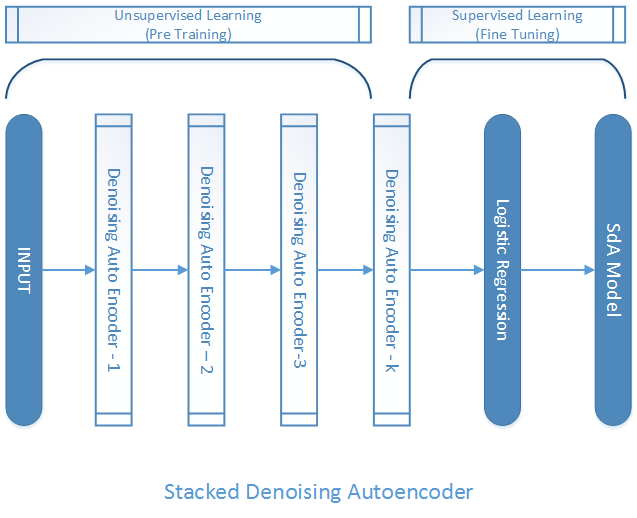
\includegraphics[width=\textwidth, height=0.6\textheight, keepaspectratio] {sda_model_stack}
\caption{Design of SdA model}
\label{fig:sda_model_stack}
\end{figure}


\section{Malware Family Classification}
\label{Multiclass Classification}
For malware family classification we setup the problem as multiclass classification problem. All benign applications are labelled as 'Clean' while malicious applications are labelled as as per there family name.  We evaluate different models for our dataset which includes RandomForest, SVM (RBF), AdaBoost and SdA. The results are discussed in Section ~\ref{Malware Detection}.

\section{Evaluation Parameters}
Here we compare the accuracy of various model for classification problem. We also calculate other The precision, accuracy, specificity, recall, F-measure for the given models are calculated as follows:

\begin{equation}\label{eq:formula}
\centering
\begin{aligned}
\bf Precision &= \frac{TP} {(TP + FP)}  \\ \nonumber
\bf Accuracy &= \frac{TP + TN} {(TP + TN + FP + FN)} \\
\bf Recall &= \frac{TP} {(TP + FN)}  \\
\bf Specificity &= \frac{TN} {(TN + FN)} \\
\bf F-measure &= \frac{2 \times Precision \times Recall} {(Precision + Recall)} \\
\end{aligned}
\end{equation}

We also use 'Receiver Operating Characteristic' (ROC) curve which illustrates the performance of a binary classifier system as its discrimination threshold is varied. It is created by plotting the fraction of true positives out of the total actual positives (TPR = true positive rate) vs. the fraction of false positives out of the total actual negatives (FPR = false positive rate), at various threshold settings. TPR is also known as sensitivity or recall.

\[
{\bf FPR = \frac{FP} {(FP + TP)}}
\]

